
\subsection{Model}
\paragraph*{Architecture}
It could be formulated as a regression problem from sequence to value: given sequence \( X \), a learned
function \( F \) could map the \( X \) to the \( y \), either retention time or ion intensity. The mathematical expression is as follows:
\[ \hat{y} = F(X;\Theta) \]
$\Theta$ is the parameters of the model.we find the optimal parameters \( \Theta^\star\) by minimizing  the loss function \( L \).
\[ \Theta^\star = \arg\min_{\Theta} L(\hat{y}, y) \]
We use the LSTM + Transformer model (illustrated in the Figure~\ref{fig:architecture}) to solve the retention time (RT) and ion intensity prediction task.
The long short-term memory (LSTM)~\cite{hochreiter1997long} module comprises of two stacks of bi-directional LSTM. For each stack of LSTM, it has two layers and the dimension of input embedding and hidden state are 256 and 512, respectively. After one stack of LSTM, a combination of LeakyReLU-dropout-linear layer is configured. LSTM is a kind of recurrent neural network(RNN) trying to use gate function to capture the long dependency in the input sequence. The bi-directional LSTM, expecting to learn a good token embedding for the network's downstream layers, is scheduled as the first module of our model.

Transformer~\cite{vaswani2017attention} is the second module composed of n Transformer encoder.
Each Transformer encoder has 8 attention head, then a feedforward layer configured after attention head.

\begin{figure}[t]
    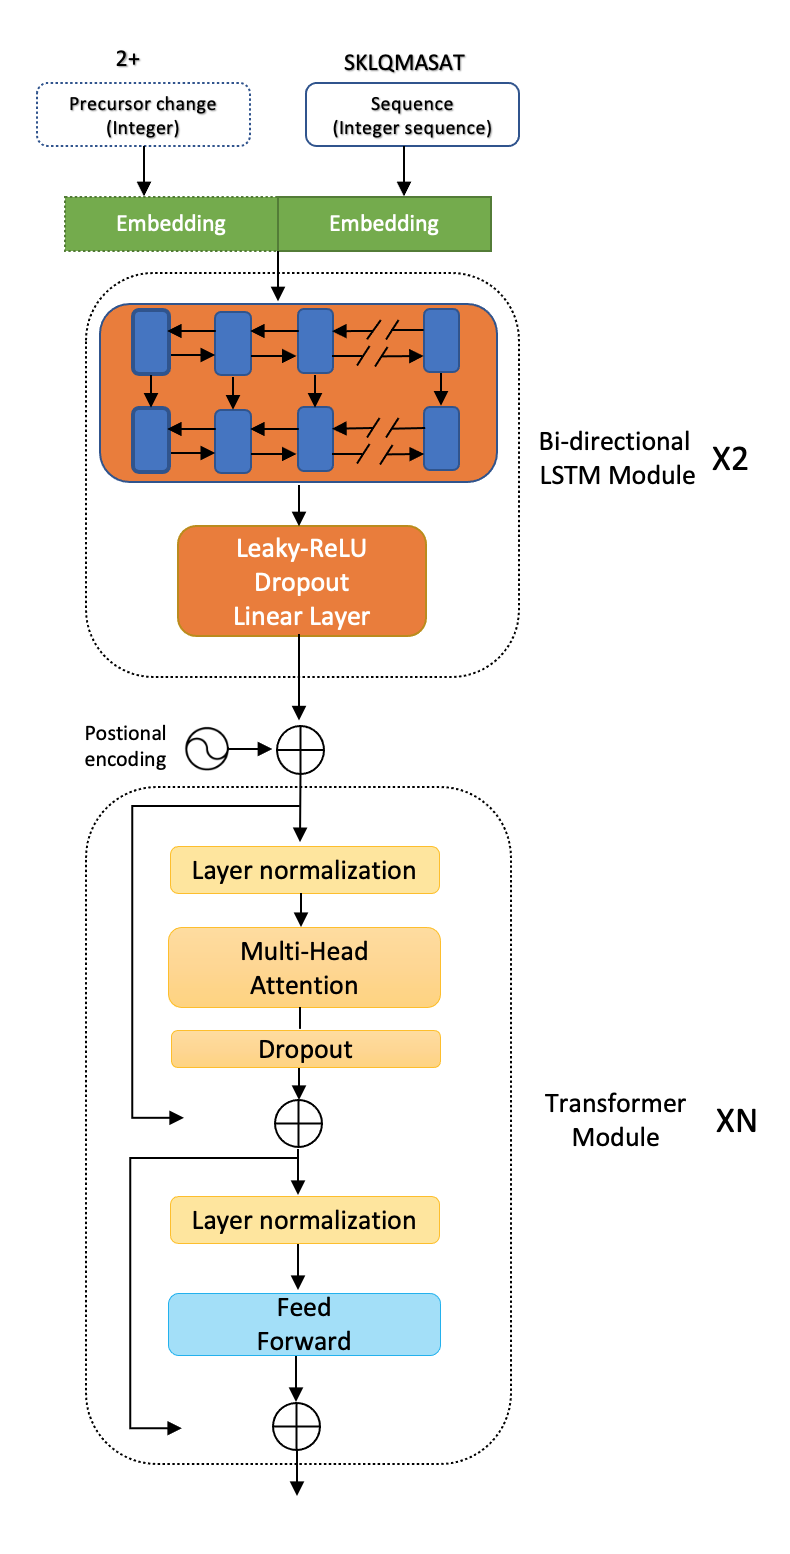
\includegraphics[width=3.5in]{arch.png}
    \caption{Model architecture}
  \label{fig:architecture}
  \end{figure}

\subsection{RT prediction}
\paragraph*{Self-attention and position encoding}
Transformer is an entirely different model by exploiting the self-attention compared to RNN.
Self-attention is an attention mechanism relating different positions of a single sequence to compute a representation of the sequence. Self-attention has been used successfully in a variety of tasks, including reading
comprehension, textual entailment, and learning task-independent sentence representations.
The Transformer is the first transduction model relying entirely on self-attention to compute its input and output representations without using sequence-aligned RNNs or convolution. It has achieved state-of-the-art performance in multiple natural language tasks, such as language translation, language entailment classification, language modeling, etc. We use the pre-layer form of Transformer, which is proposed in~\cite{xiong2020layer} and converges much faster.

The position encoding by sine and cosine functions is added to the output of LSTM module then feed into the Transformer module.
We take the same way of position encoding as~\cite{vaswani2017attention} which is as follows:
\begin{align*}
    PE_{(pos, 2i)} &= \sin{(pos/10000^{\frac{2i}{d_{model}}})} \\
    PE_{(pos, 2i+1)} &= \cos{(pos/10000^{\frac{2i}{d_{model}}})}
\end{align*}
where $pos$  is the position, $i$ is the dimension and $d_{model}$ have the same dimensions with input embeddings.



For this task, we implement
5 models with two units of two layers bi-directional LSTM and 4, 5, 6, 7, 8 Transformer encoder layers, correspondingly. We train and select those 5 models independently. After obtaining the best models, those 5 predictions of retention time are averaged as the final prediction for each peptide.

The amino acid tokens are embedded into 256 dimensions to the neural network.
Especially since the output of the Transformer is the same length as the input sequence, we need to take it down to one scaler for retention time. By adding the time distributed linear layer to assign varied weights for different amino acids dynamically, we obtain RT prediction.
Herein we use the square root of mean squared error (RMSE) as loss function.

%-------------------------------------------------------------------------
\subsection{Ion intensity prediction}

We implement one model for ion intensity prediction, which has two units of two layers bi-directional LSTM and 8 layers of Transformer encoder. Like the RT prediction task, we first embed the amino acids token, the charge to 192, 64 dimensions separately then concatenate those two vectors, forming the 256 dimension vectors to the neural network. The last layer is a linear layer, which projects the feature from high dimension to 8 dimensions with length unchanged as our prediction of ion intensity.

We use mean squared
error (MSE) as our loss function. For both RT and Ion intensity tasks, we use Adam optimizer~\cite{kingma2017adam}, and the learning rate is 1e-4, the learning rate decay at the milestone epochs during the training. We implement our models by the Python and Pytorch, and train the model on multiple GPUs. 


